\section{Tasso in presenza di distorsione}

Consideriamo ora il problema di ricostruire il canale di DL
\(\bm{h}^\mathrm{(D)}\) alla BS in presenza di una data distorsione \(d\).

Anzitutto, poiché una stima del canale di UL è già presente alla BS, possiamo
vedere lo scenario considerato come una codifica di sorgenti correlate
distribuite (i canali di UL e DL) con informazione laterale (il canale
\(\bm{h}^\mathrm{(U)}\) già noto alla BS). Desideriamo quindi utilizzare
l'informazione laterale, nota solo al decodificatore (la BS nel nostro caso),
per ridurre il tasso di trasmissione \(b_\mathrm{B}\) necessario per effettuare
una trasmissione di \(\bm{h}^\mathrm{(D)}\) che risulti affidabile anche in
presenza della suddetta distorsione \(d\). La situazione appena descritta è
rappresentata in Figura~\ref{fig:wz-configuration}.

\begin{figure}[ht]
    \centering
    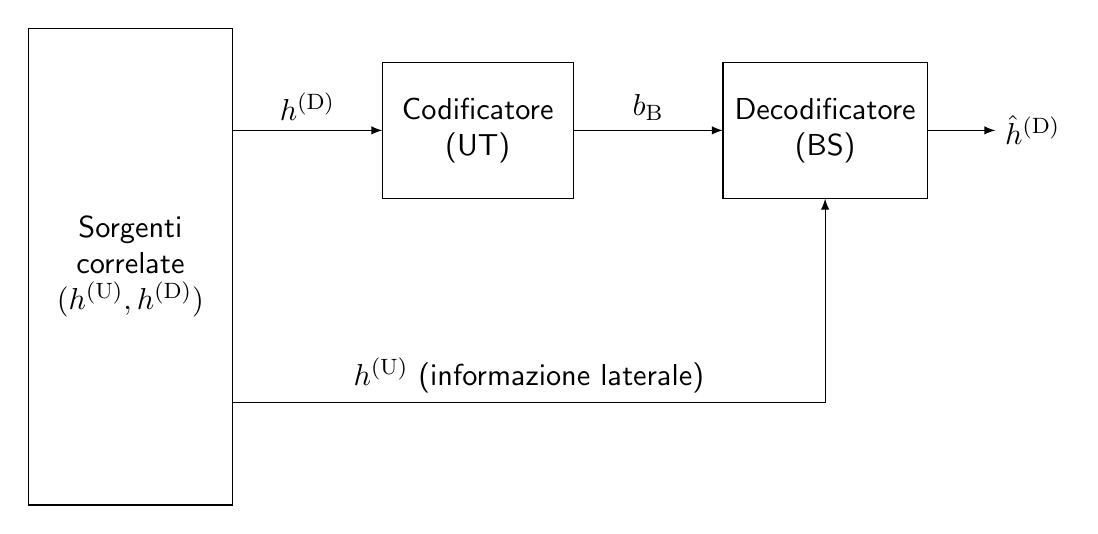
\begin{tikzpicture}[scale=0.865,>=latex]
    \tikzstyle{every node}=[font=\fontsize{11}{13}\sffamily]

    \draw (0,0) rectangle (3,7)
    node[midway,align=center]
    {Sorgenti \\ correlate \\ \((\bm{h}^\mathrm{(U)},\bm{h}^\mathrm{(D)})\)};

    \draw[->] (3,5.5) -- (5.2,5.5)
    node[above,midway]{\(\bm{h}^\mathrm{(D)}\)};

    \draw[-] (3,1.5) -- (11.7,1.5)
    node[above,midway]{\(\bm{h}^\mathrm{(U)}\) (informazione laterale)};

    \draw[->] (11.7,1.5) -- (11.7,4.5);

    \draw (5.2,4.5) rectangle (8,6.5)
    node[midway,align=center]{Codificatore \\ (UT)};

    \draw[->] (8,5.5) -- (10.2,5.5)
    node[above,midway]{\(b_\mathrm{B}\)};

    \draw (10.2,4.5) rectangle (13.2,6.5)
    node[midway,align=center]{Decodificatore \\ (BS)};

    \draw[->] (13.2,5.5) -- (14.2,5.5)
    node[right]{\(\hat{\bm{h}}^\mathrm{(D)}\)};
\end{tikzpicture}

    \caption{Configurazione per la codifica di sorgente con informazione laterale.}
    \label{fig:wz-configuration}
\end{figure}

Un'estensione del teorema di Slepian-Wolf (Teorema~\ref{thm:sw}) è possibile
grazie al lavoro di Wyner e Ziv. Di seguito, riportiamo il teorema di
Wyner-Ziv, completo di descrizione formale del problema
considerato.\cite{1055508}

\begin{thm}[Wyner-Ziv \textnormal{\cite{10.1002/047174882X.ch15}}]
    \label{thm:wz}

    Detto \(\set{U}\) un insieme finito arbitrario, sia \(\set{U}^n\) l'insieme
    dei vettori di \(n\) elementi con valori in \(\set{U}\). Denotiamo con
    \(\bm{X}^n\) un vettore aleatorio di cardinalità \(n\). Per
    \(k=1,2,\dots\), definiamo l'insieme
    \begin{equation}
        I_k = \{0,1,2,\dots,k-1\}.
    \end{equation}
    Siano \(\set{X},\set{Y},\hat{\set{X}}\) insiemi finiti e sia
    \(\{(X_k,Y_k)\}_1^\infty\) una sequenza di estrazioni indipendenti di una
    coppia di variabili aleatorie dipendenti \(X,Y\) con valori in \(\set{X}\)
    e \(\set{Y}\), rispettivamente. La distribuzione di probabilità for \(X,Y\)
    è
    \begin{equation}
        Q(x,y) = \prob{X = x, Y = y}, \quad x \in \set{X}, y \in \set{Y}.
    \end{equation}
    Sia \(D: \set{X}\times\hat{\set{X}} \to [0,\infty)\) una funzione di
    distorsione. Un codice \((n,M,\Delta)\) è definito da una coppia di
    funzioni \(F_\mathrm{E},F_\mathrm{D}\), un "codificatore" e un
    "decodificatore", rispettivamente, dove
    \begin{alignat}{1}
        F_\mathrm{E}: \set{X}^n \to I_M &, \\
        F_\mathrm{D}: \set{Y}^n \times I_M \to \hat{\set{X}}^n &,
    \end{alignat}
    e
    \begin{equation}
        \expect{\frac{1}{n} \sum_{k=1}^n D(X_k,\hat{X}_k)} = \Delta,
    \end{equation}
    dove \(\hat{\bm{X}}^n = F_\mathrm{D}(\bm{Y}^n,F_\mathrm{E}(\bm{X}^n))\).
    Diciamo che una coppia \((R,d)\) è ottenibile se, per \(\varepsilon > 0\) a
    piacere, esiste (per \(n\) sufficientemente grande) un codice
    \((n,M,\Delta)\) con
    \begin{equation}
        M \le 2^{n (R + \varepsilon)}, \quad \Delta \le d + \varepsilon .
    \end{equation}
    Definiamo con \(\set{R}\) l'insieme delle coppie \((R,d)\) ottenibili, e
    definiamo
    \begin{equation}
        R^{*}(d) = \min_{(R,d)\,\in\,\set{R}} R . \label{eq:r-star}
    \end{equation}
    Poiché, per la definizione data, \(\set{R}\) è un insieme chiuso, il minimo
    indicato nella definizione di \(R^{*}(d)\) esiste. Inoltre, dal momento che
    \(R^{*}(d)\) è una funzione non crescente in \(d\), abbiamo \(R^{*}(0) \ge
    \lim_{d\to0} R^{*}(d)\). Per di più, dalla \eqref{eq:r-star}, per tutti i
    valori di \(d \ge 0\), la coppia \((R^{*}(d), d) \in \set{R}\). Infine, dal
    momento che \(\set{R}\) è chiuso, \((\lim_{d\to0} R^{*}(d), 0) \in
    \set{R}\), e abbiamo che \(R^{*}(0) \le \lim_{d\to0} R^{*}(d)\).
    Concludiamo quindi che \(R^{*}(d)\) è continua in \(d = 0\).

    Sia \(p(x,y,z), x \in \set{X}, y \in \set{Y}, z \in \set{Z}\), dove
    \(\set{Z}\) è un insieme finito arbitrario, una distribuzione di
    probabilità che definisce le variabili aleatorie \(X,Y,Z\), tali che la
    distribuzione marginale per \(X,Y\) è
    \begin{equation}
        \sum_{z \in \set{Z}} p(x,y,z) = Q(x,y) \label{eq:wz-distr-constr-1}
    \end{equation}
    e tale che
    \begin{equation}
        Y,Z \textrm{ sono condizionate indipendentemente data } X.
        \label{eq:wz-distr-constr-2}
    \end{equation}
    Ora, per \(d > 0\), definiamo \(\set{M}(d)\) come l'insieme delle
    distribuzioni di probabilità \(p(x,y,z)\) che soddisfa
    \eqref{eq:wz-distr-constr-1} e \eqref{eq:wz-distr-constr-2}, e che ha la
    proprietà che esiste una funzione \(f: \set{Y}\times\set{X} \to
    \hat{\set{X}}\) tale che
    \begin{equation}
        \expect{D(X,\hat{X})} \le d, \quad
        \textrm{dove } \hat{X} = f(Y,Z) .
    \end{equation}
    Definiamo infine, per \(d > 0\), la quantità
    \begin{equation}
        \bar{R}(d) \define \inf_{p\,\in\,\set{M}(d)} \mleft[
            \mutual{X}{Z} - \mutual{Y}{Z}
            \mright] .
    \end{equation}
    Poiché \(\set{M}(d)\) è una funzione non crescente in \(d\), \(\bar{R}(d)\)
    è non crescente, per \(d \in (0,\infty)\). Quindi, possiamo definire
    \begin{equation}
        \bar{R}(0) = \lim_{d\to0} \bar{R}(d) .
    \end{equation}
    Si ha, per \(d \ge 0\), \(R^{*}(d) = \bar{R}(d)\) .
\end{thm}

Il teorema di Wyner-Ziv ci dice quindi che, in presenza di distorsione \(d\),
possiamo effettuare la trasmissione del canale di DL dallo UT alla BS con un
tasso
\begin{equation}
    b_\mathrm{B} \ge \inf_{p\,\in\,\set{M}(d)}
    \mutual{\bm{h}^{(D)}}{Z \given \bm{h}^{(U)}} , \label{eq:rate-with-wz}
\end{equation}
dove la variabile aleatoria ausiliaria \(Z \in \set{Z}\), con \(\set{Z}\)
insieme finito, deve soddisfare i vincoli: i) \(\bm{h}^{(U)},Z\) condizionate
indipendentemente dato \(\bm{h}^{(D)}\); ii) esiste una funzione \(f:
\set{V}\times\set{Z} \to \hat{\set{D}}\), tale che
\(\expect{D(\bm{h}^{(D)},f(\bm{h}^{(U)},Z))} \le d\), dove \(\hat{\set{D}}\) è
l'alfabeto in cui prende valori la versione ricevuta alla BS del canale di DL.

Nella pratica, risultati simili al limite teorico \eqref{eq:rate-with-wz} si
possono ottenere, ad esempio, utilizzando una codifica tramite sindrome che
sfrutti la presenza dell'informazione laterale, ovvero la stima di
\(\bm{h}^{(U)}\) nota al decodificatore, la BS. A questo proposito, si veda il
lavoro di S.S. Pradhan e K. Ramachandran.\cite{1184140}
